\chapter{Probability and Counting}

\section{Introduction}

We will start with some basic definitions.

\begin{definition}[Sample Space]
    The sample space \(\Omega\) is the set of all possible outcomes
\end{definition}

For example, when flipping three coins, we have \(2^3 = 8\) outcomes:
\[
    \Omega = \{\text{HHH}, \text{HHT}, \text{HTH}, \text{HTT}, \text{THH}, \text{THT}, \text{TTH}, \text{TTT}\}
\]

\begin{definition}[Event]
    An event is a subset of the sample space.
\end{definition}

Following the above example, if \(A\) is the event that at least two heads occur, we have:
\[
    A = \{\text{HHH}, \text{HHT}, \text{HTH}, \text{THH}\}
\]

\begin{definition}
    The probability of an event is the sum of the probability of its outcomes. 
    \begin{itemize}
        \item Probabilities are non-negative.
        \item Probabilities add up to one.
    \end{itemize}
\end{definition}

Again from the above example, we see that the probability of each event is equal to \(\frac{1}{8}\), and they can be summed up to 1. 

\begin{definition}
    The probability of an event is the sum of the probabilities of its outcomes.
\end{definition}

For event \(A\), the probability would be 
\[
    \mathbb{P}(A) = \dfrac{1}{8} + \dfrac{1}{8} + \dfrac{1}{8} + \dfrac{1}{8} = \dfrac{1}{2}
\]

\begin{proposition}[Uniform Probability Law]
    If the outcomes in \(\Omega\) are equally likely, then the probability of event \(A\) will be 
    \[
        \mathbb{P}(A) = \dfrac{\text{Number of outcomes in }A}{\text{Number of outcomes in }\Omega} = \dfrac{\vert A \vert}{\vert \Omega \vert}
    \]

    \begin{remark}
        It can only be used when every outcome is equally likely.
    \end{remark}
\end{proposition}

For event \(A\), the probability would be 
\[
    \mathbb{P}(A) = \dfrac{\vert A \vert}{\vert \Omega \vert} = \dfrac{4}{8} = \dfrac{1}{2}
\]

\begin{eg}
We roll two dice. Which of the following outcome is more likely for the sum of the two dice?

1. 11

2. 12

3. equally likely

\textbf{Solution:} 
For the sum to be 11, we can have (5, 6) and (6, 5). However, for the sum to be 12, we can only have (6, 6). Therefore, for \(\vert \Omega \vert = 6^2 = 36\),
\[
    \mathbb{P}(11) = \dfrac{2}{36},\quad\mathbb{P}(12) = \dfrac{1}{36}
\]
Therefore, the sum of 11 would be more likely to occur. 
\end{eg}

\section{Permutation and Combination}

\subsection{Counting via Product Rule}
\begin{proposition}[Product Rule]
    Suppose there are \(n\) possible outcomes for Experiment 1 and \(m\) possible outcomes for Experiment 2, where the two experiments are independent. Then, there are \(m \times n\) possible outcomes for the two experiments.
\end{proposition}

For example, when flipping three coins, each of them has two possible outcomes. Therefore, there are in total \(2 \times 2 \times 2 = 8\) possible outcomes. 

We can then generalize this rule for cases that the outcomes of experiment 1 may affect the outcomes of experiment 2.
\begin{proposition}[Generalized Product Rule]
    Suppose that
    \begin{itemize}
        \item There are \(n\) possible outcomes for Experiment 1. 
        \item For every outcome of Experiment 1, there are \(m\) possible outcomes for Experiment 2.
    \end{itemize}
    Then, there are \(m \times n\) possible outcomes for the two experiments.
\end{proposition}

For example, when finding all possible outcomes for rolling two dice with different values, the outcomes of the first experiment, i.e. rolling the first die, would be 6. The outcomes of the second experiment, i.e. rolling the second die, would be 5 (since we need to exclude the outcome of the first die). Then, there are in total \(6 \times 5 = 30\) possible outcomes. 

\begin{eg}
    We roll two dice. What is the probability that they come out with different values?
    
    \textbf{Solution:}
    Let \(A\) be the desired event. Then we have
    \[
        \mathbb{P}(A) = \dfrac{\vert A \vert}{\vert \Omega \vert} = \dfrac{6 \times 5}{6 \times 6} = \dfrac{5}{6}
    \]
\end{eg}

\begin{eg}
    We roll two dice. What is the probability that the sum of dice equals 7? What is the probability that the sum of dice is an odd number?

    \textbf{Solution: }
    Let \(A\) be the event that the sum of dice equals 7. Then we have
    \[
        A = \{(1, 6), (2, 5), \cdots, (6, 1)\}
    \]
    \[
        \mathbb{P}(A) = \dfrac{\vert A \vert }{\vert \Omega \vert } = \dfrac{6}{6^2} = \dfrac{1}{6}
    \]
    Let \(B\) be the event that the sum of dice is an odd number. Then we have
    \[
        B = \{(1, 2), (1, 4), \cdots, (6, 5)\},\quad \vert B \vert = 6 \times 3,
    \]
    where for each number in the first die, there will be exactly three numbers in the second die that can be added up to an odd number. Thus,
    \[
        \mathbb{P}(B) = \dfrac{\vert B \vert }{\vert \Omega \vert } = \dfrac{6 \times 3}{6^2} = \dfrac{1}{2}
    \]
\end{eg}

\begin{eg}
    We again roll two dice. What is the probability that the first die is bigger than the second die?

    \textbf{Solution: }
    In this case, we cannot use generalized product rule since for every outcome in the first experiment, there will be a different outcome in the second experiment. Let \(A\) be the desired event. Then we have 
    \[
        A = \{(2, 1), (3, 1), \cdots, (6, 5)\}
    \]
    \[
        \mathbb{P}(A) = \dfrac{\vert A \vert }{\vert \Omega \vert } = \dfrac{15}{6^2} = \dfrac{5}{12}
    \]
\end{eg}

\subsection{Permutation}

\begin{definition}[Permutation]
    A permutation of \(n\) different objects is an arrangement of the objects into an ordered sequence (order matters).
\end{definition}

\begin{proposition}
    For \(n\) different objects, there exists \(n!\) different permutations:
    \[
        n! = n \times (n-1) \times \cdots \times 2 \times 1
    \]
\end{proposition}

\begin{eg}
    We roll six dice. How many ways are there for the six dice to have different values? What is the probability of that event?
    
    \textbf{Solution:}
    Let \(A\) be the desired event. Then we have
    \[
        \vert A \vert = 6 \times 5 \times 4 \times 3 \times 2 \times 1 = 6! = 720, \quad \mathbb{P}(A) = \dfrac{\vert A \vert }{\vert \Omega \vert } = \dfrac{6!}{6^6}
    \]
\end{eg}

\begin{eg}[Birthday Paradox]
    Suppose there are \(n\) people in a room. We assume that a year only has 365 days, and that every day is equally likely to be the birthday of a person. What is the probability that at least two people have the same birthday? Here we assume that \(n < 365\). 

    For sample space \(S\) we have the set of all possible sequences of \(n\) birthday, the \(\vert S \vert = 365^n\). 

    Let \(T\) be the event in which at least two birthdays are the same. Then we have
    \[
        \mathbb{P}(T) = 1 - \dfrac{365 \times 364 \times \cdots \times (365 - n + 1)}{365^n},
    \]
    where the term \((365 \times 364 \times \cdots \times (365 - n + 1))\) is to count the possible outcomes for the event that all birthdays are distinct.
\end{eg}
Birthday paradox could be visualized as below:
\begin{figure}[H]
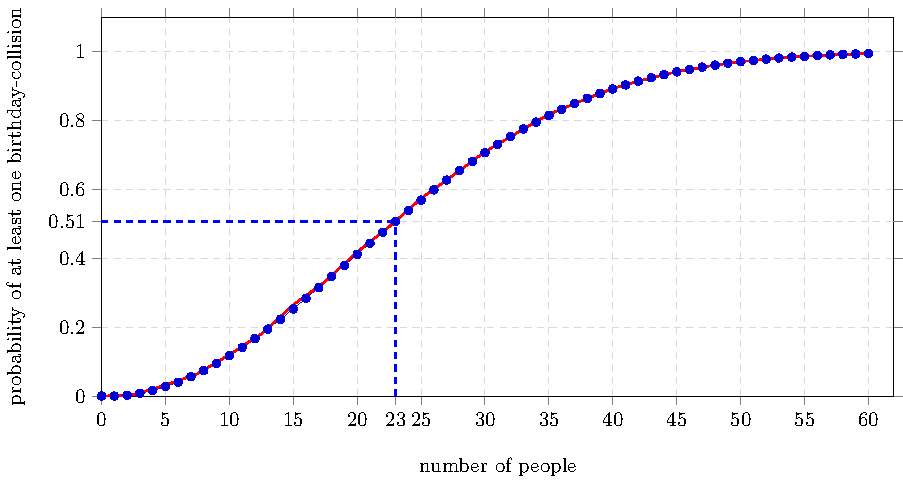
\includegraphics{Figures/Birthday_paradox.pdf}
\caption*{Adapted from \href{https://github.com/MartinThoma/LaTeX-examples/tree/2286e6e3833904b2c058b2a855db9b7f81776c59/tikz/birthday-paradox}{MartinThoma}}
\end{figure}

\subsection{Binomial Coefficient}
\begin{proposition}[Binomial Coefficient or "\(n\)-Choose-\(k\)"]
    Given a set \(S\) of size \(n\), the number of subsets of size \(k\) will be 
    \[
        \binom{n}{k} = \dfrac{n!}{k!(n-k)!}
    \]
    It can also be understood as the number of possible arrangements of \(k\) objects of Type A and \(n - k\) objects of Type B into an ordered sequence.
\end{proposition}

\begin{eg}
    A box contains 8 red balls and 2 blue balls. You draw 2 balls at random(without replacement). What is the probability that the two balls have different colors?

    \textbf{Solution:}
    Let \(A\) be the desired event.
    \[
        \mathbb{P}(A) = \dfrac{\vert A \vert}{\vert \Omega \vert} = \dfrac{\binom{8}{1}\binom{2}{1}}{\binom{10}{2}} = \dfrac{16}{45}
    \]
\end{eg}

\begin{proposition}[Multinomial Coefficient]
    For a set \(S\) of size \(n\), the number of partitioning of the set to partitions of size \(k_1, k_2, \cdots, k_t\) (noted that \(n = k_1 + k_2 + \cdots + k_t\)) will be
    \[
        \binom{n}{k_1, k_2, \cdots, k_t} = \dfrac{n!}{k_1!k_2!\cdots k_t!}
    \]
    It can also be understood as the number of possible permutations of \(k_1\) objects of Type 1, \(k_2\) objects of Type 2, ..., and \(k_t\) objects of Type \(t\).
\end{proposition}

% END OF DOCUMENT